\documentclass[11pt, a4paper]{article}
\usepackage[utf8]{inputenc}
\usepackage[left=3cm, right=3cm, top=2.5cm, bottom=3.0cm]{geometry}
\usepackage{amsmath, amssymb, amsthm}
\usepackage[english]{babel}
\usepackage{graphicx}
\usepackage[font={small,it}]{caption}
\graphicspath{ {figures/} }
\usepackage{url}
\usepackage{multirow}
\usepackage{titling}
\usepackage{subcaption}
\usepackage{wrapfig}
\usepackage{appendix}
\usepackage{float}
\usepackage[bottom]{footmisc}
\usepackage{titling}
%\setlength{\droptitle}{-10em}  

\title{ \huge Artificial Neural Networks \\ 
  { \large Project 1: Regression and Classification with MLPs }}
\author{
        Lood, Cédric \\
        \small Master of Bioinformatics
}

\begin{document}
\maketitle
%\tableofcontents

\section{Context}

The analysis presented in this report was done for the class of
Artificial Neural Networks at KU Leuven (Spring 2016). It consists in
practical implementations of Multi-layer perceptrons (MLP) to solve
regression and classification problems in a supervised setting, with a
brief foray into unsupervised learning for dimensionality
reduction. The implementation was done in the MatLab environment
(2015a) using the neural networks toolbox. The scripts for each of the
sections can be found in the annex to this report.

\section{Regression}

\begin{wrapfigure}{r}{0.5\textwidth}
  \vspace{-20pt}
  \centering
  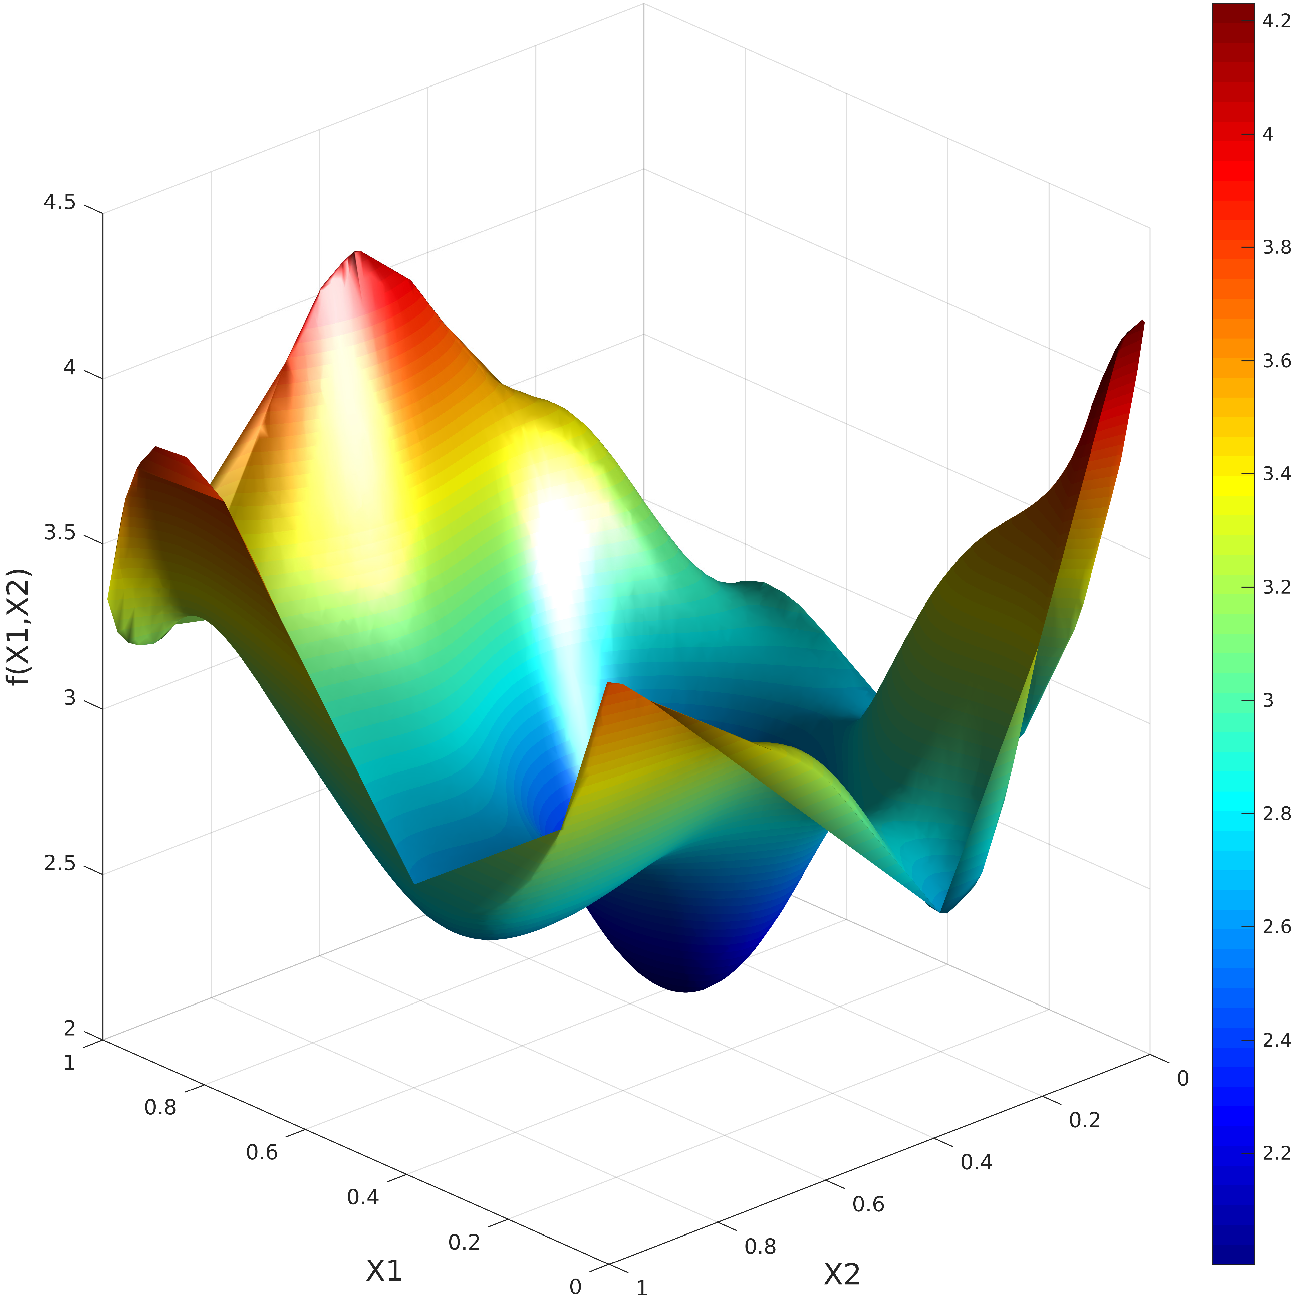
\includegraphics[scale=.35]{regression_dataset.pdf}
  \caption{Visualization of the full dataset}
  \label{fig:regression_dataset}
\end{wrapfigure}

% \begin{wrapfigure}{r}{0.5\textwidth}
%   \vspace{-20pt}
%   \begin{center}
%     \includegraphics[width=0.48\textwidth]{gull}
%   \end{center}
%   \vspace{-20pt}
%   \caption{A gull}
%   \vspace{-10pt}
% \end{wrapfigure}

The problem we need to solve here is to estimate a (unknown)
non-linear function from a given dataset of 13600 datapoints uniformly
sampled. Importantly to note, the sampled data is noiseless. The
dependent variable was generated using the student number (r0575791)
and the two dependent variables $X_1, X_2 \in [0, 1]$ (figure
\ref{fig:regression_dataset} for a rendering of the dataset
generated).

For the creation of the training, validation, and test set, I first
randomized the dataset and then proceeded to use the built-in matlab
function \emph{dividerand} which creates 3 lists of non-repeating
indices of size 1000 that can then be used to subset the original
dataset into the 3 subsets. The visualization of the sets on figure
\ref{fig:regression_traindataset} reassures that the sampling was done
correctly.

Although it is possible to use more than one layer for MLPs, I limited
myself here at 1 hidden layer, comforted by the fact that they consist
of universal approximator given that I used a non-linear transfer
function. I also obtained good results previously (see homework 1) for
function approximation using a single hidden layer. The choices I was
faced with to optimize the architecture are the number of hidden
units, the transfer function, and the choice of the training
algorithm. For the rest, the network has 2 input neurons connected to
the hidden neurons, whose outputs are linearly combined by a single
output neuron.

\begin{figure}[H]
%\vspace{-20pt}
  \centering
  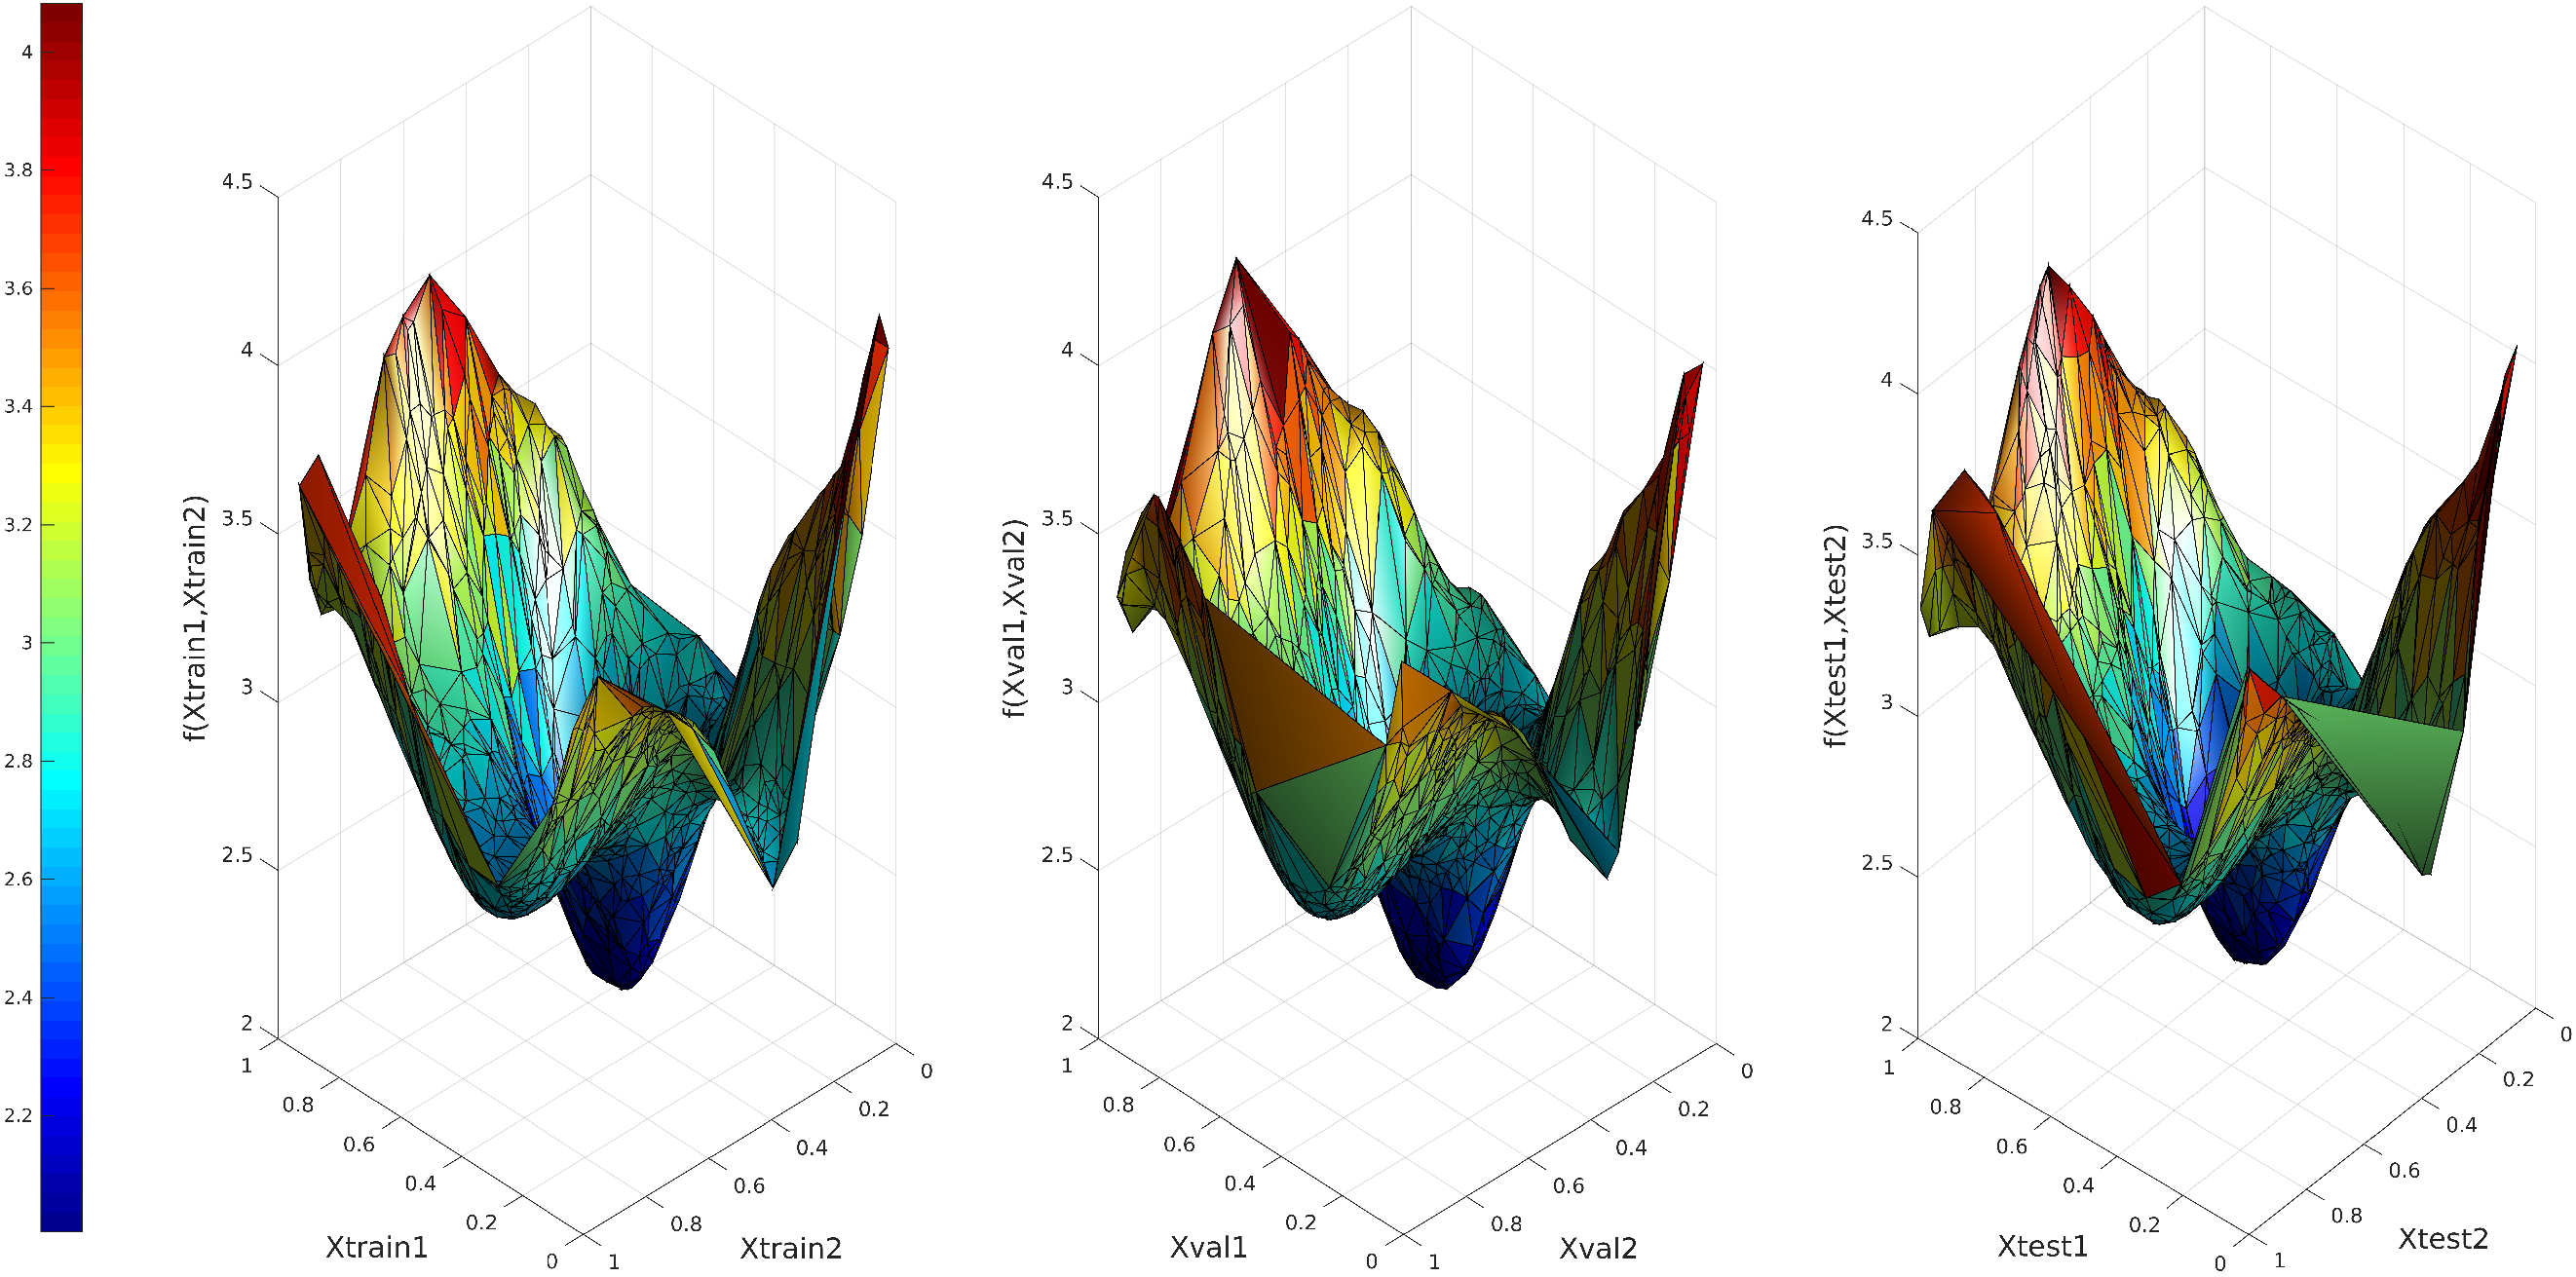
\includegraphics[scale=.30]{regression_trainingsets.pdf}
  \caption{From left to right: training, validation, and test datasets
    (1000 points each)}
  \label{fig:regression_traindataset}
\end{figure}

For the training algorithm, I based my choice on consideration such as
the size of the dataset. Since I worked on an interactive computing
node of the VSC \footnote{Vlaams Super Computer}, I did not have to
worry to much about the memory requirements (even though a 1000x1000
Hessian matrix can also be handled by a laptop computer without any
troubles), and did not investigate conjugate gradient
methods. Instead, I chose to focus on the Levenberg-Marquardt method,
which is known for its fast convergence.

On the figure \ref{fig:test_mse_error}, I report the finding in terms
of validation MSE (no usage of the training set at this stage). I
performed a systematic search for the correct amount of hidden neurons
using \emph{transig} and \emph{logsig}. On the same figure, the Test
MSE for the selected architecture of 60 hidden neurons, and a
\emph{tansig} transfer function is reported.

\begin{figure}[H]
  \centering
  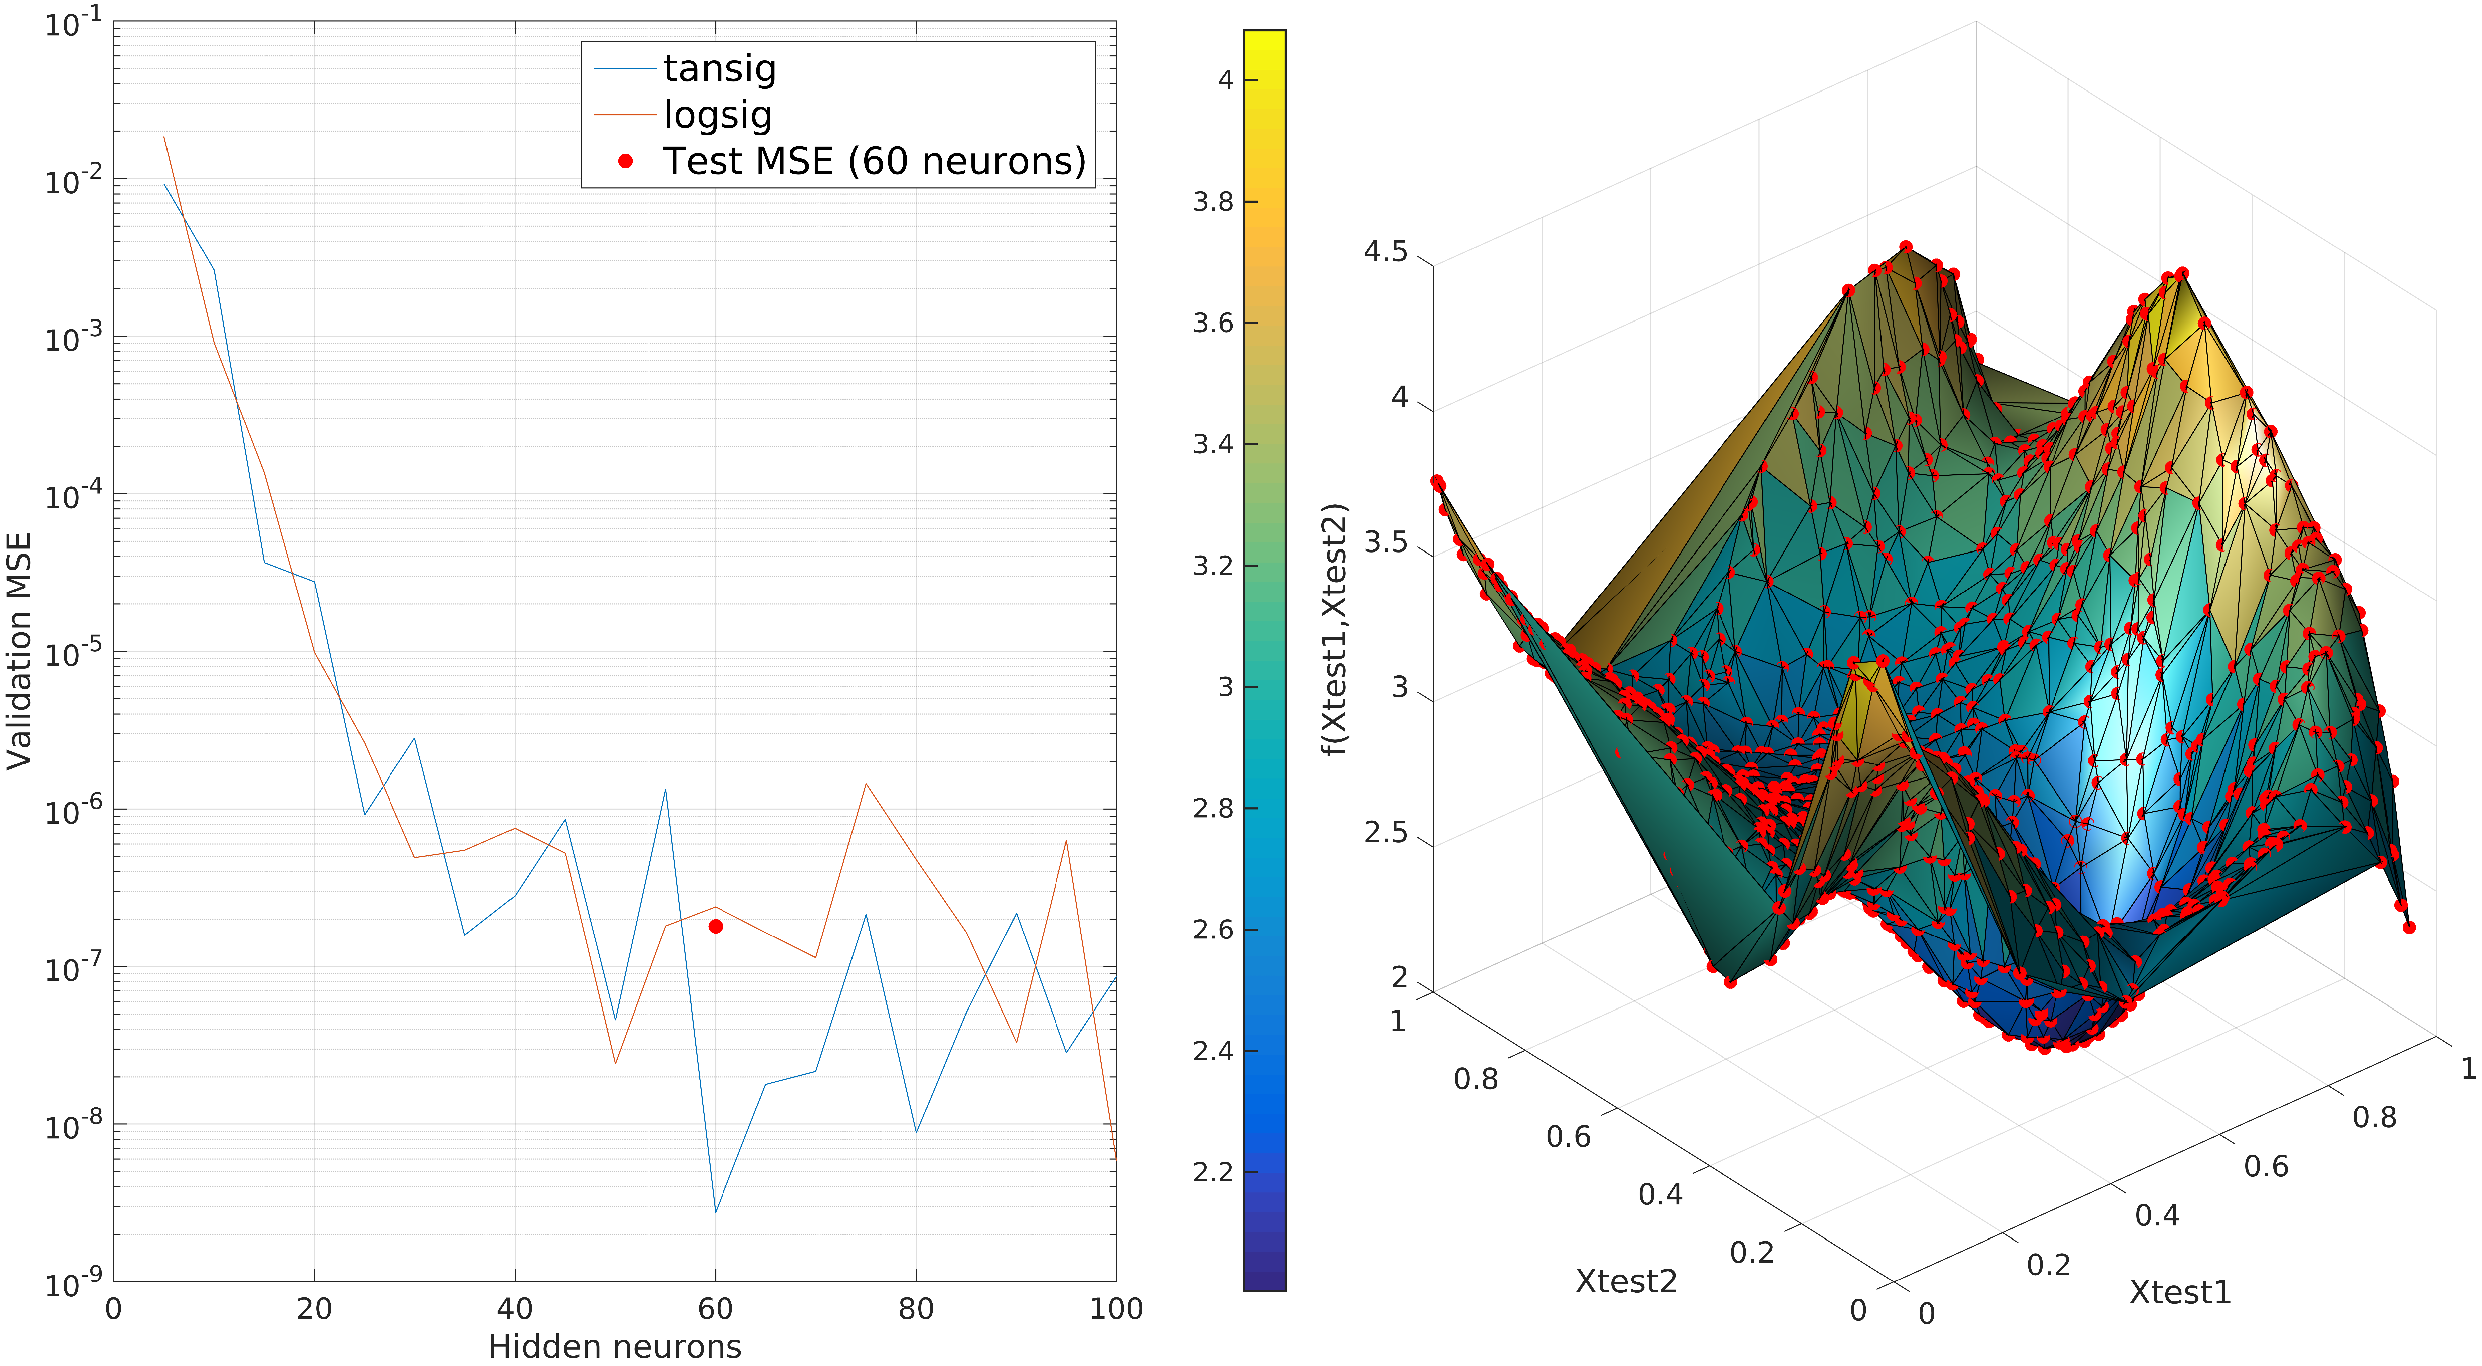
\includegraphics[scale=0.34]{regression_logtan_error.pdf}
  \caption{Validation MSE curves and test surface + prediction (red balls)}
  \label{fig:test_mse_error}
\end{figure}

Computation of the difference between the predicted values and actual
values for the test set revealed the extreme precision of the function
estimation. The errors are in the order of $10^-5$ to $10^-9$, the
largest error (in absolute value) is 0.015. Although this is indeed
excellent, it is possible to improve the process by using more of the
available data. Using cross validation on 80\% of the dataset for
example and set aside 20\% of the dataset for test purposes.

\section{Classification}

% \begin{figure}[H]
%   \centering
%   \includegraphics[scale=.43]{training_performance.pdf}
%   \caption{Training performance}
%   \label{fig:trainnl}
% \end{figure}

%{\footnotesize
%\bibliographystyle{ieeetr} 
%\bibliography{bib-db}}

\end{document}
